\documentclass[12pt,a4paper]{article}

\usepackage[a4paper,text={16.5cm,25.2cm},centering]{geometry}
\usepackage{lmodern}
\usepackage{amssymb,amsmath}
\usepackage{bm}
\usepackage{graphicx}
\usepackage{microtype}
\usepackage{hyperref}
\setlength{\parindent}{0pt}
\setlength{\parskip}{1.2ex}

\hypersetup
       {   pdfauthor = { Gilberto Boareto \& Daniel Coutinho },
           pdftitle={ A Julia Implementation of Gensys },
           colorlinks=TRUE,
           linkcolor=black,
           citecolor=blue,
           urlcolor=blue
       }

\title{ A Julia Implementation of Gensys }

\author{ Gilberto Boareto \& Daniel Coutinho }

\date{ October, 2019 }

\usepackage{upquote}
\usepackage{listings}
\usepackage{xcolor}
\lstset{
    basicstyle=\ttfamily\footnotesize,
    upquote=true,
    breaklines=true,
    breakindent=0pt,
    keepspaces=true,
    showspaces=false,
    columns=fullflexible,
    showtabs=false,
    showstringspaces=false,
    escapeinside={(*@}{@*)},
    extendedchars=true,
}
\newcommand{\HLJLt}[1]{#1}
\newcommand{\HLJLw}[1]{#1}
\newcommand{\HLJLe}[1]{#1}
\newcommand{\HLJLeB}[1]{#1}
\newcommand{\HLJLo}[1]{#1}
\newcommand{\HLJLk}[1]{\textcolor[RGB]{148,91,176}{\textbf{#1}}}
\newcommand{\HLJLkc}[1]{\textcolor[RGB]{59,151,46}{\textit{#1}}}
\newcommand{\HLJLkd}[1]{\textcolor[RGB]{214,102,97}{\textit{#1}}}
\newcommand{\HLJLkn}[1]{\textcolor[RGB]{148,91,176}{\textbf{#1}}}
\newcommand{\HLJLkp}[1]{\textcolor[RGB]{148,91,176}{\textbf{#1}}}
\newcommand{\HLJLkr}[1]{\textcolor[RGB]{148,91,176}{\textbf{#1}}}
\newcommand{\HLJLkt}[1]{\textcolor[RGB]{148,91,176}{\textbf{#1}}}
\newcommand{\HLJLn}[1]{#1}
\newcommand{\HLJLna}[1]{#1}
\newcommand{\HLJLnb}[1]{#1}
\newcommand{\HLJLnbp}[1]{#1}
\newcommand{\HLJLnc}[1]{#1}
\newcommand{\HLJLncB}[1]{#1}
\newcommand{\HLJLnd}[1]{\textcolor[RGB]{214,102,97}{#1}}
\newcommand{\HLJLne}[1]{#1}
\newcommand{\HLJLneB}[1]{#1}
\newcommand{\HLJLnf}[1]{\textcolor[RGB]{66,102,213}{#1}}
\newcommand{\HLJLnfm}[1]{\textcolor[RGB]{66,102,213}{#1}}
\newcommand{\HLJLnp}[1]{#1}
\newcommand{\HLJLnl}[1]{#1}
\newcommand{\HLJLnn}[1]{#1}
\newcommand{\HLJLno}[1]{#1}
\newcommand{\HLJLnt}[1]{#1}
\newcommand{\HLJLnv}[1]{#1}
\newcommand{\HLJLnvc}[1]{#1}
\newcommand{\HLJLnvg}[1]{#1}
\newcommand{\HLJLnvi}[1]{#1}
\newcommand{\HLJLnvm}[1]{#1}
\newcommand{\HLJLl}[1]{#1}
\newcommand{\HLJLld}[1]{\textcolor[RGB]{148,91,176}{\textit{#1}}}
\newcommand{\HLJLs}[1]{\textcolor[RGB]{201,61,57}{#1}}
\newcommand{\HLJLsa}[1]{\textcolor[RGB]{201,61,57}{#1}}
\newcommand{\HLJLsb}[1]{\textcolor[RGB]{201,61,57}{#1}}
\newcommand{\HLJLsc}[1]{\textcolor[RGB]{201,61,57}{#1}}
\newcommand{\HLJLsd}[1]{\textcolor[RGB]{201,61,57}{#1}}
\newcommand{\HLJLsdB}[1]{\textcolor[RGB]{201,61,57}{#1}}
\newcommand{\HLJLsdC}[1]{\textcolor[RGB]{201,61,57}{#1}}
\newcommand{\HLJLse}[1]{\textcolor[RGB]{59,151,46}{#1}}
\newcommand{\HLJLsh}[1]{\textcolor[RGB]{201,61,57}{#1}}
\newcommand{\HLJLsi}[1]{#1}
\newcommand{\HLJLso}[1]{\textcolor[RGB]{201,61,57}{#1}}
\newcommand{\HLJLsr}[1]{\textcolor[RGB]{201,61,57}{#1}}
\newcommand{\HLJLss}[1]{\textcolor[RGB]{201,61,57}{#1}}
\newcommand{\HLJLssB}[1]{\textcolor[RGB]{201,61,57}{#1}}
\newcommand{\HLJLnB}[1]{\textcolor[RGB]{59,151,46}{#1}}
\newcommand{\HLJLnbB}[1]{\textcolor[RGB]{59,151,46}{#1}}
\newcommand{\HLJLnfB}[1]{\textcolor[RGB]{59,151,46}{#1}}
\newcommand{\HLJLnh}[1]{\textcolor[RGB]{59,151,46}{#1}}
\newcommand{\HLJLni}[1]{\textcolor[RGB]{59,151,46}{#1}}
\newcommand{\HLJLnil}[1]{\textcolor[RGB]{59,151,46}{#1}}
\newcommand{\HLJLnoB}[1]{\textcolor[RGB]{59,151,46}{#1}}
\newcommand{\HLJLoB}[1]{\textcolor[RGB]{102,102,102}{\textbf{#1}}}
\newcommand{\HLJLow}[1]{\textcolor[RGB]{102,102,102}{\textbf{#1}}}
\newcommand{\HLJLp}[1]{#1}
\newcommand{\HLJLc}[1]{\textcolor[RGB]{153,153,119}{\textit{#1}}}
\newcommand{\HLJLch}[1]{\textcolor[RGB]{153,153,119}{\textit{#1}}}
\newcommand{\HLJLcm}[1]{\textcolor[RGB]{153,153,119}{\textit{#1}}}
\newcommand{\HLJLcp}[1]{\textcolor[RGB]{153,153,119}{\textit{#1}}}
\newcommand{\HLJLcpB}[1]{\textcolor[RGB]{153,153,119}{\textit{#1}}}
\newcommand{\HLJLcs}[1]{\textcolor[RGB]{153,153,119}{\textit{#1}}}
\newcommand{\HLJLcsB}[1]{\textcolor[RGB]{153,153,119}{\textit{#1}}}
\newcommand{\HLJLg}[1]{#1}
\newcommand{\HLJLgd}[1]{#1}
\newcommand{\HLJLge}[1]{#1}
\newcommand{\HLJLgeB}[1]{#1}
\newcommand{\HLJLgh}[1]{#1}
\newcommand{\HLJLgi}[1]{#1}
\newcommand{\HLJLgo}[1]{#1}
\newcommand{\HLJLgp}[1]{#1}
\newcommand{\HLJLgs}[1]{#1}
\newcommand{\HLJLgsB}[1]{#1}
\newcommand{\HLJLgt}[1]{#1}


\begin{document}

\maketitle

\section{Introduction}
This document is a white paper on our implementation of gensys, the solution method developed by Sims (2002). Our implementation follows closely Sims's paper and the description in Miao (2014). In general, one takes a model written as:

\[
\Gamma_0 y_t = \Gamma_1 y_{t-1} + \Psi \varepsilon_t + \Pi \eta_t
\]
In which $y_t$ are the variables today, $\varepsilon_t$ is a vector of exogenous shocks and $\eta_t$ is a vector of endogenous errors, i.e. expectational errors.

Sims's method allows for a $\Gamma_0$ that is singular. Instead of determining some variables as \emph{jump} and others as \emph{predetermined}, as Blanchard and Khan (1980) or Klein (2000), Sims's allows it to be done endogenously by the algorithm.

Sims's method has another remarkable difference from the previous methods: instead of "root counting" - checking that the number of eigenvalues larger than 1 equals the number of \emph{jump} variables and the number of eigenvalues smaller than 1 equals the number of \emph{predetermined} variables - Sims's algorithm relies on ensuring that the expectational errors are linear combinations of the exogenous shocks. We will go into more details in the next section.

We implement this in Julia. Julia is a modern programming language focused on scientific computing, trying to balance speed and ease to use. Julia has reached maturity only recently. However, there is a large number of packages written for Julia. Thomas Sargent is probably the most famous economist with ties with Julia, dedicating a whole section of his website to the language and how-to solve standard models in economics using Julia - although this does not include large scale DSGEs. \href{https://juliacomputing.com/case-studies/ny-fed.html}{The Federal Reserve Bank of New York (FED-NY) implemented their DSGE on Julia.} By their own account, this sped up estimation ten fold and solving the model was eleven times faster. Given the time it takes to estimate even a medium DSGE model, these gains are not negligibles. Moreover, Julia has a large numerical linear algebra library that comes out of the box (you don't need to install anything besides Julia). This is valuable given that we will work with \emph{linear} models.

This white paper is divided as follows: in the next section, we briefly discuss two methods of numerical linear algebra that will be used in our implementation: the Schur Decomposition (also called the QZ decomposition) and the Singular Value Decomposition (SVD); section three concisely presents the algorithm and our implementation; section four presents a small example from Gali (2008), which has analytical solution - this allows us to make sure that our implementation is sound; section five concludes.

\section{Numerical Linear Algebra}
We will use two decompositions of matrices: the Schur Decomposition and the Singular Value Decomposition (SVD). Both are closely related to the more well known eigenvalue decomposition:

\[
A = P^{-1}\Lambda P
\]
In which $\Lambda$ is a diagonal matrix. In general, $P$ is not orthonormal. The eigenvectors matrix, $P$, is orthonormal, i.e. $P^{-1} = P'$ in some cases, for example, if A is normal (Symmetric matrices are normal).

The Schur Decomposition tries to find a decomposition	of the same form of the eigenvalue decomposition, but instead of imposing that $\Lambda$ is diagonal, we now want that P\$ be orthonormal. So the Schur Decomposition then finds:

\[
A = Q'SQ
\]
Remarkably $S$ is always an upper triangular matrix.

We will be actually interested in the Generalized Schur Decomposition. To understand this one, lets first understand what is the generalized eigenvalue. In the usual eigenvalue problem, we want to find a vector $\mathbf{x}$ and a value $\lambda$ such that:

\[
Ax = \lambda x
\]
Rewritting this in matricial terms, we want:

\[
(A - \lambda I)x = 0
\]
In which $I$ stands for the identity matrix. Now, what if we want to solve the following problem:

\[
Ax = \lambda{}Bx
\]
We can find matrices such that $B = P^{-1}P$ and $A = P^{-1}\Lambda{}P$, in which $\Lambda$ is a diagonal matrix.

The idea for the Generalized Schur Decomposition will be the same, but now we want to find matrices $Q,Z,S,T$ such that:

\begin{itemize}
\item[1. ] \[
Q
\]
and $Z$ are orthonormal


\item[2. ] \[
S
\]
and $T$ are upper triangular


\item[3. ] \[
A = QSZ
\]

\item[4. ] \[
B = QTZ
\]

\item[5. ] \[
\forall i
\]
$S_{ii}, T_{ii}$ are not zero


\item[6. ] The pairs $(S_{ii}, T_{ii})$ can be arranged in any order

\end{itemize}
Item 6 will be particularly useful in what follows

The SVD also follows the idea from the eigenvalue problem. Now the idea is to decompose A as $USV'$, in which S is a diagonal matrix and both $U$ and $V$ are orthonormal.

\section{An example}
As a proof of concept, lets compare our code with the model of Gali (2008), chapter 3 - this is the simplest standard New Keynesian Model. Lets load first our code for Gensys:


\begin{lstlisting}
(*@\HLJLk{using}@*) (*@\HLJLn{Plots}@*)

(*@\HLJLnf{include}@*)(*@\HLJLp{(}@*)(*@\HLJLnf{string}@*)(*@\HLJLp{(}@*)(*@\HLJLnf{pwd}@*)(*@\HLJLp{(),}@*) (*@\HLJLs{"{}/src/gensys.jl"{}}@*)(*@\HLJLp{))}@*)
\end{lstlisting}

\begin{lstlisting}
irf (generic function with 2 methods)
\end{lstlisting}


We also loaded the library Plots. We will calibrate exactly as Gali does, on page 52:


\begin{lstlisting}
(*@\HLJLn{bet}@*) (*@\HLJLoB{=}@*) (*@\HLJLnfB{0.99}@*)
(*@\HLJLn{sig}@*) (*@\HLJLoB{=}@*) (*@\HLJLni{1}@*)
(*@\HLJLn{phi}@*) (*@\HLJLoB{=}@*) (*@\HLJLni{1}@*)
(*@\HLJLn{alfa}@*) (*@\HLJLoB{=}@*) (*@\HLJLni{1}@*)(*@\HLJLoB{/}@*)(*@\HLJLni{3}@*)
(*@\HLJLn{epsilon}@*) (*@\HLJLoB{=}@*) (*@\HLJLni{6}@*)
(*@\HLJLn{theta}@*) (*@\HLJLoB{=}@*) (*@\HLJLni{2}@*)(*@\HLJLoB{/}@*)(*@\HLJLni{3}@*)
(*@\HLJLn{phi{\_}pi}@*) (*@\HLJLoB{=}@*) (*@\HLJLnfB{1.5}@*)
(*@\HLJLn{phi{\_}y}@*) (*@\HLJLoB{=}@*) (*@\HLJLnfB{0.5}@*)(*@\HLJLoB{/}@*)(*@\HLJLni{4}@*)
(*@\HLJLn{rho{\_}v}@*) (*@\HLJLoB{=}@*) (*@\HLJLnfB{0.5}@*)

(*@\HLJLn{THETA}@*) (*@\HLJLoB{=}@*) (*@\HLJLp{(}@*)(*@\HLJLni{1}@*)(*@\HLJLoB{-}@*)(*@\HLJLn{alfa}@*)(*@\HLJLp{)}@*)(*@\HLJLoB{/}@*)(*@\HLJLp{(}@*)(*@\HLJLni{1}@*)(*@\HLJLoB{-}@*)(*@\HLJLn{alfa}@*)(*@\HLJLoB{+}@*)(*@\HLJLn{alfa}@*)(*@\HLJLoB{*}@*)(*@\HLJLn{epsilon}@*)(*@\HLJLp{)}@*)
(*@\HLJLn{lamb}@*) (*@\HLJLoB{=}@*) (*@\HLJLp{(}@*)(*@\HLJLni{1}@*)(*@\HLJLoB{-}@*)(*@\HLJLn{theta}@*)(*@\HLJLp{)}@*)(*@\HLJLoB{*}@*)(*@\HLJLp{(}@*)(*@\HLJLni{1}@*)(*@\HLJLoB{-}@*)(*@\HLJLn{bet}@*)(*@\HLJLoB{*}@*)(*@\HLJLn{theta}@*)(*@\HLJLp{)}@*)(*@\HLJLoB{/}@*)(*@\HLJLn{theta}@*)(*@\HLJLoB{*}@*)(*@\HLJLn{THETA}@*)
(*@\HLJLn{kappa}@*) (*@\HLJLoB{=}@*) (*@\HLJLn{lamb}@*)(*@\HLJLoB{*}@*)(*@\HLJLp{(}@*)(*@\HLJLn{sig}@*)(*@\HLJLoB{+}@*)(*@\HLJLp{(}@*)(*@\HLJLn{phi}@*)(*@\HLJLoB{+}@*)(*@\HLJLn{alfa}@*)(*@\HLJLp{)}@*)(*@\HLJLoB{/}@*)(*@\HLJLp{(}@*)(*@\HLJLni{1}@*)(*@\HLJLoB{-}@*)(*@\HLJLn{alfa}@*)(*@\HLJLp{))}@*)
\end{lstlisting}

\begin{lstlisting}
0.12750000000000006
\end{lstlisting}


We refer the reader to Gali's book for knowing what each parameter means. Next, we need to write the usual model in Sim's format. Let us repeat the three equations of the usual model:

\[
\pi_t = \beta E_t(\pi_{t+1}) + \kappa \tilde{y}_t\\
\tilde{y}_t = -\frac{1}{\sigma} (i_t - E_t(\pi_{t+1})) + E_t(\tilde{y}_{t+1})\\
i_t = \phi_{\pi} \pi_t + \phi_{\tilde{y}} \tilde{y}_t + v_t\\
v_t = \rho_v v_{t-1} + \varepsilon_t^v
\]
Gali's book gives an analytical solution for the impulse response functions for a shock $v_t$. This can be found on page 51. We implement them in Julia as well:


\begin{lstlisting}
(*@\HLJLn{LAMBDA{\_}v}@*) (*@\HLJLoB{=}@*) (*@\HLJLp{((}@*)(*@\HLJLni{1}@*)(*@\HLJLoB{-}@*)(*@\HLJLn{bet}@*)(*@\HLJLoB{*}@*)(*@\HLJLn{rho{\_}v}@*)(*@\HLJLp{)}@*)(*@\HLJLoB{*}@*)(*@\HLJLp{(}@*)(*@\HLJLn{sig}@*)(*@\HLJLoB{*}@*)(*@\HLJLp{(}@*)(*@\HLJLni{1}@*)(*@\HLJLoB{-}@*)(*@\HLJLn{rho{\_}v}@*)(*@\HLJLp{)}@*)(*@\HLJLoB{+}@*)(*@\HLJLn{phi{\_}y}@*)(*@\HLJLp{)}@*)(*@\HLJLoB{+}@*)(*@\HLJLn{kappa}@*)(*@\HLJLoB{*}@*)(*@\HLJLp{(}@*)(*@\HLJLn{phi{\_}pi}@*)(*@\HLJLoB{-}@*)(*@\HLJLn{rho{\_}v}@*)(*@\HLJLp{))}@*)(*@\HLJLoB{{\textasciicircum}}@*)(*@\HLJLp{(}@*)(*@\HLJLoB{-}@*)(*@\HLJLni{1}@*)(*@\HLJLp{)}@*)

(*@\HLJLnf{y{\_}irf}@*)(*@\HLJLp{(}@*)(*@\HLJLn{v}@*)(*@\HLJLp{)}@*) (*@\HLJLoB{=}@*) (*@\HLJLoB{-}@*)(*@\HLJLp{(}@*)(*@\HLJLni{1}@*)(*@\HLJLoB{-}@*)(*@\HLJLn{bet}@*)(*@\HLJLoB{*}@*)(*@\HLJLn{rho{\_}v}@*)(*@\HLJLp{)}@*)(*@\HLJLoB{*}@*)(*@\HLJLn{LAMBDA{\_}v}@*)(*@\HLJLoB{*}@*)(*@\HLJLn{v}@*)
(*@\HLJLnf{pi{\_}irf}@*)(*@\HLJLp{(}@*)(*@\HLJLn{v}@*)(*@\HLJLp{)}@*) (*@\HLJLoB{=}@*) (*@\HLJLoB{-}@*)(*@\HLJLn{kappa}@*)(*@\HLJLoB{*}@*)(*@\HLJLn{LAMBDA{\_}v}@*)(*@\HLJLoB{*}@*)(*@\HLJLn{v}@*)
(*@\HLJLnf{r{\_}irf}@*)(*@\HLJLp{(}@*)(*@\HLJLn{v}@*)(*@\HLJLp{)}@*) (*@\HLJLoB{=}@*) (*@\HLJLn{sig}@*)(*@\HLJLoB{*}@*)(*@\HLJLp{(}@*)(*@\HLJLni{1}@*)(*@\HLJLoB{-}@*)(*@\HLJLn{rho{\_}v}@*)(*@\HLJLp{)}@*)(*@\HLJLoB{*}@*)(*@\HLJLp{(}@*)(*@\HLJLni{1}@*)(*@\HLJLoB{-}@*)(*@\HLJLn{bet}@*)(*@\HLJLoB{*}@*)(*@\HLJLn{rho{\_}v}@*)(*@\HLJLp{)}@*)(*@\HLJLoB{*}@*)(*@\HLJLn{LAMBDA{\_}v}@*)(*@\HLJLoB{*}@*)(*@\HLJLn{v}@*)
(*@\HLJLnf{i{\_}irf}@*)(*@\HLJLp{(}@*)(*@\HLJLn{v}@*)(*@\HLJLp{)}@*) (*@\HLJLoB{=}@*) (*@\HLJLp{(}@*)(*@\HLJLn{sig}@*)(*@\HLJLoB{*}@*)(*@\HLJLp{(}@*)(*@\HLJLni{1}@*)(*@\HLJLoB{-}@*)(*@\HLJLn{rho{\_}v}@*)(*@\HLJLp{)}@*)(*@\HLJLoB{*}@*)(*@\HLJLp{(}@*)(*@\HLJLni{1}@*)(*@\HLJLoB{-}@*)(*@\HLJLn{bet}@*)(*@\HLJLoB{*}@*)(*@\HLJLn{rho{\_}v}@*)(*@\HLJLp{)}@*) (*@\HLJLoB{-}@*) (*@\HLJLn{rho{\_}v}@*)(*@\HLJLoB{*}@*)(*@\HLJLn{kappa}@*)(*@\HLJLp{)}@*)(*@\HLJLoB{*}@*)(*@\HLJLn{LAMBDA{\_}v}@*)(*@\HLJLoB{*}@*)(*@\HLJLn{v}@*)
(*@\HLJLnf{v}@*)(*@\HLJLp{(}@*)(*@\HLJLn{v}@*)(*@\HLJLp{,}@*)(*@\HLJLn{uu}@*)(*@\HLJLp{)}@*) (*@\HLJLoB{=}@*) (*@\HLJLn{rho{\_}v}@*)(*@\HLJLoB{*}@*)(*@\HLJLn{v}@*) (*@\HLJLoB{+}@*) (*@\HLJLn{uu}@*)
\end{lstlisting}

\begin{lstlisting}
v (generic function with 1 method)
\end{lstlisting}


And we compute a sample IRF for a positive 25 basis shock in the interest rate:


\begin{lstlisting}
(*@\HLJLn{irfs{\_}true}@*) (*@\HLJLoB{=}@*) (*@\HLJLnf{zeros}@*)(*@\HLJLp{(}@*)(*@\HLJLni{15}@*)(*@\HLJLp{,}@*)(*@\HLJLni{5}@*)(*@\HLJLp{)}@*)

(*@\HLJLn{irfs{\_}true}@*)(*@\HLJLp{[}@*)(*@\HLJLni{1}@*)(*@\HLJLp{,}@*)(*@\HLJLni{1}@*)(*@\HLJLp{]}@*) (*@\HLJLoB{=}@*) (*@\HLJLni{0}@*)

(*@\HLJLn{uu}@*) (*@\HLJLoB{=}@*) (*@\HLJLnfB{0.25}@*)

(*@\HLJLk{for}@*) (*@\HLJLn{t}@*) (*@\HLJLkp{in}@*) (*@\HLJLni{2}@*)(*@\HLJLoB{:}@*)(*@\HLJLni{15}@*)
    (*@\HLJLn{irfs{\_}true}@*)(*@\HLJLp{[}@*)(*@\HLJLn{t}@*)(*@\HLJLp{,}@*)(*@\HLJLni{4}@*)(*@\HLJLp{]}@*) (*@\HLJLoB{=}@*) (*@\HLJLnf{v}@*)(*@\HLJLp{(}@*)(*@\HLJLn{irfs{\_}true}@*)(*@\HLJLp{[}@*)(*@\HLJLn{t}@*)(*@\HLJLoB{-}@*)(*@\HLJLni{1}@*)(*@\HLJLp{,}@*)(*@\HLJLni{4}@*)(*@\HLJLp{],}@*)(*@\HLJLn{uu}@*)(*@\HLJLp{)}@*)
    (*@\HLJLn{irfs{\_}true}@*)(*@\HLJLp{[}@*)(*@\HLJLn{t}@*)(*@\HLJLp{,}@*)(*@\HLJLni{1}@*)(*@\HLJLp{]}@*) (*@\HLJLoB{=}@*) (*@\HLJLnf{pi{\_}irf}@*)(*@\HLJLp{(}@*)(*@\HLJLn{irfs{\_}true}@*)(*@\HLJLp{[}@*)(*@\HLJLn{t}@*)(*@\HLJLp{,}@*)(*@\HLJLni{4}@*)(*@\HLJLp{])}@*)
    (*@\HLJLn{irfs{\_}true}@*)(*@\HLJLp{[}@*)(*@\HLJLn{t}@*)(*@\HLJLp{,}@*)(*@\HLJLni{2}@*)(*@\HLJLp{]}@*) (*@\HLJLoB{=}@*) (*@\HLJLnf{y{\_}irf}@*)(*@\HLJLp{(}@*)(*@\HLJLn{irfs{\_}true}@*)(*@\HLJLp{[}@*)(*@\HLJLn{t}@*)(*@\HLJLp{,}@*)(*@\HLJLni{4}@*)(*@\HLJLp{])}@*)
    (*@\HLJLn{irfs{\_}true}@*)(*@\HLJLp{[}@*)(*@\HLJLn{t}@*)(*@\HLJLp{,}@*)(*@\HLJLni{3}@*)(*@\HLJLp{]}@*) (*@\HLJLoB{=}@*) (*@\HLJLnf{i{\_}irf}@*)(*@\HLJLp{(}@*)(*@\HLJLn{irfs{\_}true}@*)(*@\HLJLp{[}@*)(*@\HLJLn{t}@*)(*@\HLJLp{,}@*)(*@\HLJLni{4}@*)(*@\HLJLp{])}@*)
    (*@\HLJLn{irfs{\_}true}@*)(*@\HLJLp{[}@*)(*@\HLJLn{t}@*)(*@\HLJLp{,}@*)(*@\HLJLni{5}@*)(*@\HLJLp{]}@*) (*@\HLJLoB{=}@*) (*@\HLJLnf{r{\_}irf}@*)(*@\HLJLp{(}@*)(*@\HLJLn{irfs{\_}true}@*)(*@\HLJLp{[}@*)(*@\HLJLn{t}@*)(*@\HLJLp{,}@*)(*@\HLJLni{4}@*)(*@\HLJLp{])}@*)
    (*@\HLJLkd{global}@*) (*@\HLJLn{uu}@*) (*@\HLJLoB{=}@*) (*@\HLJLni{0}@*)
(*@\HLJLk{end}@*)
\end{lstlisting}


Now lets solve it numerically: the first step is to write $\eta_t^{\pi} = \pi_t - E_{t-1} \pi_t$ and $\eta_t^{\tilde{y}} = \tilde{y}_t - E_{t-1} \tilde{y}_t$. Now, use this to isolate to write the expectations as function of the true value plus the expectational error - $E_t(\pi_{t+1}) = \pi_t + \eta_t^{\pi}$ for example.

This allows us to write the system above as follows:

\[
\pi_{t-1} - \kappa \tilde{y}_{t-1} + \beta \eta_t^{\pi} = \beta \pi_t\\
\sigma\tilde{y}_{t-1} + i_{t-1} + \eta_t^{\pi} + \sigma \eta_t^{\tilde{y}} = \pi_t + \sigma \tilde{y}_t\\
i_{t-1} - \phi_{\pi}\pi_{t-1} - \phi_{\tilde{y}} \tilde{y}_{t-1} - v_{t-1} = 0\\
v_t = \rho v_{t-1} + \varepsilon^v_t
\]
And it is straight foward to write the matrices $\Gamma_0$, $\Gamma_1$, $\Psi$, $\Pi$, as follows:


\begin{lstlisting}
(*@\HLJLn{GAMMA{\_}0}@*) (*@\HLJLoB{=}@*) (*@\HLJLp{[}@*)(*@\HLJLn{bet}@*)    (*@\HLJLni{0}@*)     (*@\HLJLni{0}@*)  (*@\HLJLni{0}@*)(*@\HLJLp{;}@*)
           (*@\HLJLni{1}@*)      (*@\HLJLn{sig}@*)   (*@\HLJLni{0}@*)  (*@\HLJLni{0}@*)(*@\HLJLp{;}@*)
           (*@\HLJLni{0}@*)      (*@\HLJLni{0}@*)     (*@\HLJLni{0}@*)  (*@\HLJLni{0}@*)(*@\HLJLp{;}@*)
           (*@\HLJLni{0}@*)      (*@\HLJLni{0}@*)     (*@\HLJLni{0}@*)  (*@\HLJLni{1}@*)(*@\HLJLp{]}@*)

(*@\HLJLn{GAMMA{\_}1}@*) (*@\HLJLoB{=}@*) (*@\HLJLp{[}@*)(*@\HLJLni{1}@*)      (*@\HLJLoB{-}@*)(*@\HLJLn{kappa}@*)  (*@\HLJLni{0}@*)  (*@\HLJLni{0}@*)(*@\HLJLp{;}@*)
           (*@\HLJLni{0}@*)       (*@\HLJLn{sig}@*)    (*@\HLJLni{1}@*)  (*@\HLJLni{0}@*)(*@\HLJLp{;}@*)
           (*@\HLJLoB{-}@*)(*@\HLJLn{phi{\_}pi}@*)  (*@\HLJLoB{-}@*)(*@\HLJLn{phi{\_}y}@*)  (*@\HLJLni{1}@*) (*@\HLJLoB{-}@*)(*@\HLJLni{1}@*)(*@\HLJLp{;}@*)
           (*@\HLJLni{0}@*)       (*@\HLJLni{0}@*)      (*@\HLJLni{0}@*)  (*@\HLJLn{rho{\_}v}@*)(*@\HLJLp{]}@*)

(*@\HLJLn{PSI}@*) (*@\HLJLoB{=}@*) (*@\HLJLp{[}@*)(*@\HLJLni{0}@*)(*@\HLJLp{;}@*) (*@\HLJLni{0}@*)(*@\HLJLp{;}@*) (*@\HLJLni{0}@*)(*@\HLJLp{;}@*) (*@\HLJLni{1}@*)(*@\HLJLp{]}@*)

(*@\HLJLn{PI}@*) (*@\HLJLoB{=}@*) (*@\HLJLp{[}@*)(*@\HLJLn{bet}@*)  (*@\HLJLni{0}@*)(*@\HLJLp{;}@*)
      (*@\HLJLni{1}@*)    (*@\HLJLn{sig}@*)(*@\HLJLp{;}@*)
      (*@\HLJLni{0}@*)    (*@\HLJLni{0}@*)(*@\HLJLp{;}@*)
      (*@\HLJLni{0}@*)    (*@\HLJLni{0}@*)(*@\HLJLp{]}@*)
\end{lstlisting}

\begin{lstlisting}
4(*@\ensuremath{\times}@*)2 Array{Float64,2}:
 0.99  0.0
 1.0   1.0
 0.0   0.0
 0.0   0.0
\end{lstlisting}


Here are LaTeX versions of the matrices generated automatically with the package \emph{latexify}, from the inputed matrices for Julia:


\begin{lstlisting}
(*@\HLJLk{using}@*) (*@\HLJLn{Latexify}@*)

(*@\HLJLnf{print}@*)(*@\HLJLp{(}@*)(*@\HLJLnf{string}@*)(*@\HLJLp{(}@*)(*@\HLJLs{"{}}@*)(*@\HLJLse{{\textbackslash}{\$}{\textbackslash}{\$}{\textbackslash}{\textbackslash}}@*)(*@\HLJLs{Gamma{\_}0}@*) (*@\HLJLs{=}@*) (*@\HLJLse{{\textbackslash}{\$}{\textbackslash}{\$}}@*)(*@\HLJLs{"{}}@*)(*@\HLJLp{,}@*)(*@\HLJLnf{latexify}@*)(*@\HLJLp{(}@*)(*@\HLJLn{GAMMA{\_}0}@*)(*@\HLJLp{)))}@*)
\end{lstlisting}

$$\Gamma_0 = $$\begin{equation}
\left[
\begin{array}{cccc}
0.99 & 0.0 & 0.0 & 0.0 \\
1.0 & 1.0 & 0.0 & 0.0 \\
0.0 & 0.0 & 0.0 & 0.0 \\
0.0 & 0.0 & 0.0 & 1.0 \\
\end{array}
\right]
\end{equation}


\begin{lstlisting}
(*@\HLJLnf{print}@*)(*@\HLJLp{(}@*)(*@\HLJLnf{string}@*)(*@\HLJLp{(}@*)(*@\HLJLs{"{}}@*)(*@\HLJLse{{\textbackslash}{\$}{\textbackslash}{\$}{\textbackslash}{\textbackslash}}@*)(*@\HLJLs{Gamma{\_}1}@*) (*@\HLJLs{=}@*) (*@\HLJLse{{\textbackslash}{\$}{\textbackslash}{\$}}@*)(*@\HLJLs{"{}}@*)(*@\HLJLp{,}@*)(*@\HLJLnf{latexify}@*)(*@\HLJLp{(}@*)(*@\HLJLn{GAMMA{\_}1}@*)(*@\HLJLp{)))}@*)
\end{lstlisting}

$$\Gamma_1 = $$\begin{equation}
\left[
\begin{array}{cccc}
1.0 & -0.12750000000000006 & 0.0 & 0.0 \\
0.0 & 1.0 & 1.0 & 0.0 \\
-1.5 & -0.125 & 1.0 & -1.0 \\
0.0 & 0.0 & 0.0 & 0.5 \\
\end{array}
\right]
\end{equation}


\begin{lstlisting}
(*@\HLJLnf{print}@*)(*@\HLJLp{(}@*)(*@\HLJLnf{string}@*)(*@\HLJLp{(}@*)(*@\HLJLs{"{}}@*)(*@\HLJLse{{\textbackslash}{\$}{\textbackslash}{\$}{\textbackslash}{\textbackslash}}@*)(*@\HLJLs{Psi}@*) (*@\HLJLs{=}@*) (*@\HLJLse{{\textbackslash}{\$}{\textbackslash}{\$}}@*)(*@\HLJLs{"{}}@*)(*@\HLJLp{,}@*)(*@\HLJLnf{latexify}@*)(*@\HLJLp{(}@*)(*@\HLJLn{PSI}@*)(*@\HLJLp{)))}@*)
\end{lstlisting}

$$\Psi = $$\begin{equation}
\left[
\begin{array}{c}
0 \\
0 \\
0 \\
1 \\
\end{array}
\right]
\end{equation}


\begin{lstlisting}
(*@\HLJLnf{print}@*)(*@\HLJLp{(}@*)(*@\HLJLnf{string}@*)(*@\HLJLp{(}@*)(*@\HLJLs{"{}}@*)(*@\HLJLse{{\textbackslash}{\$}{\textbackslash}{\$}{\textbackslash}{\textbackslash}}@*)(*@\HLJLs{Pi}@*) (*@\HLJLs{=}@*) (*@\HLJLse{{\textbackslash}{\$}{\textbackslash}{\$}}@*)(*@\HLJLs{"{}}@*)(*@\HLJLp{,}@*)(*@\HLJLnf{latexify}@*)(*@\HLJLp{(}@*)(*@\HLJLn{PI}@*)(*@\HLJLp{)))}@*)
\end{lstlisting}

$$\Pi = $$\begin{equation}
\left[
\begin{array}{cc}
0.99 & 0.0 \\
1.0 & 1.0 \\
0.0 & 0.0 \\
0.0 & 0.0 \\
\end{array}
\right]
\end{equation}


And we just call the function with this matrices:


\begin{lstlisting}
(*@\HLJLn{sol}@*) (*@\HLJLoB{=}@*) (*@\HLJLnf{gensys}@*)(*@\HLJLp{(}@*)(*@\HLJLn{GAMMA{\_}0}@*)(*@\HLJLp{,}@*)(*@\HLJLn{GAMMA{\_}1}@*)(*@\HLJLp{,}@*)(*@\HLJLn{PSI}@*)(*@\HLJLp{,}@*)(*@\HLJLn{PI}@*)(*@\HLJLp{)}@*)

(*@\HLJLn{irfs}@*) (*@\HLJLoB{=}@*) (*@\HLJLnf{irf}@*)(*@\HLJLp{(}@*)(*@\HLJLn{sol}@*)(*@\HLJLp{,}@*)(*@\HLJLni{15}@*)(*@\HLJLp{,}@*)(*@\HLJLnfB{0.25}@*)(*@\HLJLp{)}@*)
\end{lstlisting}

\begin{lstlisting}
16(*@\ensuremath{\times}@*)4 Array{Float64,2}:
 -0.0719323    -0.284908     0.106488     0.25       
 -0.0359661    -0.142454     0.053244     0.125      
 -0.0179831    -0.0712271    0.026622     0.0625     
 -0.00899154   -0.0356135    0.013311     0.03125    
 -0.00449577   -0.0178068    0.0066555    0.015625   
 -0.00224788   -0.00890339   0.00332775   0.0078125  
 -0.00112394   -0.00445169   0.00166388   0.00390625 
 -0.000561971  -0.00222585   0.000831938  0.00195312 
 -0.000280986  -0.00111292   0.000415969  0.000976562
 -0.000140493  -0.000556462  0.000207984  0.000488281
 -7.02464e-5   -0.000278231  0.000103992  0.000244141
 -3.51232e-5   -0.000139115  5.19961e-5   0.00012207 
 -1.75616e-5   -6.95577e-5   2.5998e-5    6.10352e-5 
 -8.7808e-6    -3.47788e-5   1.2999e-5    3.05176e-5 
 -4.3904e-6    -1.73894e-5   6.49951e-6   1.52588e-5 
 -2.1952e-6    -8.69471e-6   3.24976e-6   7.62939e-6
\end{lstlisting}


Lets compare the IRFs generated analyticaly and by our implementation of Gensys:


\begin{lstlisting}
(*@\HLJLnf{plot}@*)(*@\HLJLp{(}@*)(*@\HLJLni{4}@*)(*@\HLJLoB{*}@*)(*@\HLJLn{irfs}@*)(*@\HLJLp{[}@*)(*@\HLJLoB{:}@*)(*@\HLJLp{,}@*)(*@\HLJLni{1}@*)(*@\HLJLp{],}@*) (*@\HLJLn{label}@*) (*@\HLJLoB{=}@*) (*@\HLJLs{"{}Inflation}@*) (*@\HLJLs{Gensys"{}}@*)(*@\HLJLp{,}@*) (*@\HLJLn{w}@*) (*@\HLJLoB{=}@*)(*@\HLJLni{3}@*)(*@\HLJLp{)}@*)
(*@\HLJLnf{plot!}@*)(*@\HLJLp{(}@*)(*@\HLJLni{4}@*)(*@\HLJLoB{*}@*)(*@\HLJLn{irfs{\_}true}@*)(*@\HLJLp{[}@*)(*@\HLJLni{2}@*)(*@\HLJLoB{:}@*)(*@\HLJLni{15}@*)(*@\HLJLp{,}@*)(*@\HLJLni{1}@*)(*@\HLJLp{],}@*) (*@\HLJLn{label}@*) (*@\HLJLoB{=}@*) (*@\HLJLs{"{}Inflation}@*) (*@\HLJLs{Analytical"{}}@*)(*@\HLJLp{,}@*) (*@\HLJLn{line}@*) (*@\HLJLoB{=}@*) (*@\HLJLsc{:dash}@*)(*@\HLJLp{,}@*) (*@\HLJLn{w}@*) (*@\HLJLoB{=}@*)(*@\HLJLni{3}@*)(*@\HLJLp{)}@*)
(*@\HLJLnf{title!}@*)(*@\HLJLp{(}@*)(*@\HLJLs{"{}Inflation}@*) (*@\HLJLs{response}@*) (*@\HLJLs{for}@*) (*@\HLJLs{a}@*) (*@\HLJLs{0.25}@*) (*@\HLJLs{shock}@*) (*@\HLJLs{in}@*) (*@\HLJLs{interest}@*) (*@\HLJLs{rate"{}}@*)(*@\HLJLp{)}@*)
\end{lstlisting}

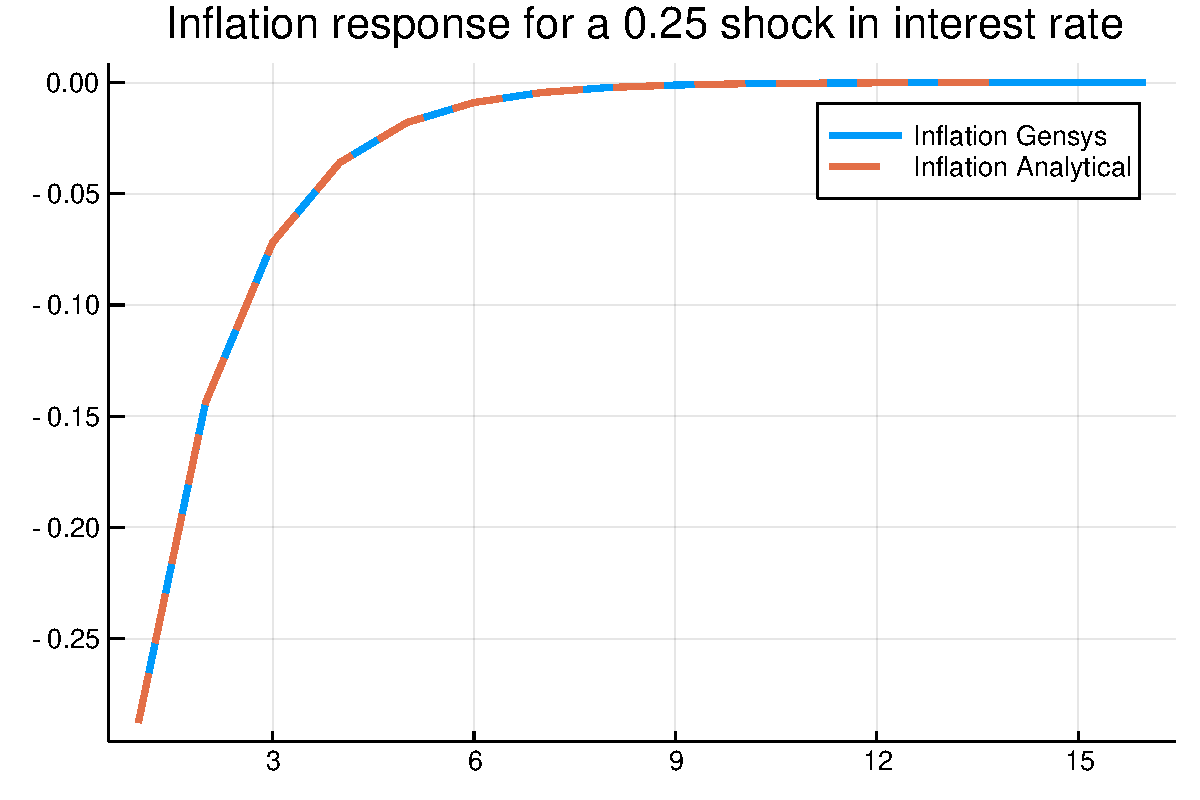
\includegraphics[width=\linewidth]{figures/gensys_11_1.pdf}

\begin{lstlisting}
(*@\HLJLnf{plot}@*)(*@\HLJLp{(}@*)(*@\HLJLn{irfs}@*)(*@\HLJLp{[}@*)(*@\HLJLoB{:}@*)(*@\HLJLp{,}@*)(*@\HLJLni{2}@*)(*@\HLJLp{],}@*) (*@\HLJLn{label}@*) (*@\HLJLoB{=}@*) (*@\HLJLs{"{}Output}@*) (*@\HLJLs{Gap}@*) (*@\HLJLs{Gensys"{}}@*)(*@\HLJLp{,}@*) (*@\HLJLn{w}@*) (*@\HLJLoB{=}@*) (*@\HLJLni{3}@*)(*@\HLJLp{)}@*)
(*@\HLJLnf{plot!}@*)(*@\HLJLp{(}@*)(*@\HLJLn{irfs{\_}true}@*)(*@\HLJLp{[}@*)(*@\HLJLni{2}@*)(*@\HLJLoB{:}@*)(*@\HLJLni{15}@*)(*@\HLJLp{,}@*)(*@\HLJLni{2}@*)(*@\HLJLp{],}@*) (*@\HLJLn{label}@*) (*@\HLJLoB{=}@*) (*@\HLJLs{"{}Output}@*) (*@\HLJLs{Gap}@*) (*@\HLJLs{Analytical"{}}@*)(*@\HLJLp{,}@*) (*@\HLJLn{line}@*) (*@\HLJLoB{=}@*) (*@\HLJLsc{:dash}@*)(*@\HLJLp{,}@*) (*@\HLJLn{w}@*) (*@\HLJLoB{=}@*) (*@\HLJLni{3}@*)(*@\HLJLp{)}@*)
(*@\HLJLnf{title!}@*)(*@\HLJLp{(}@*)(*@\HLJLs{"{}Output}@*) (*@\HLJLs{Gap}@*) (*@\HLJLs{response}@*) (*@\HLJLs{for}@*) (*@\HLJLs{a}@*) (*@\HLJLs{0.25}@*) (*@\HLJLs{shock}@*) (*@\HLJLs{in}@*) (*@\HLJLs{interest}@*) (*@\HLJLs{rate"{}}@*)(*@\HLJLp{)}@*)
\end{lstlisting}

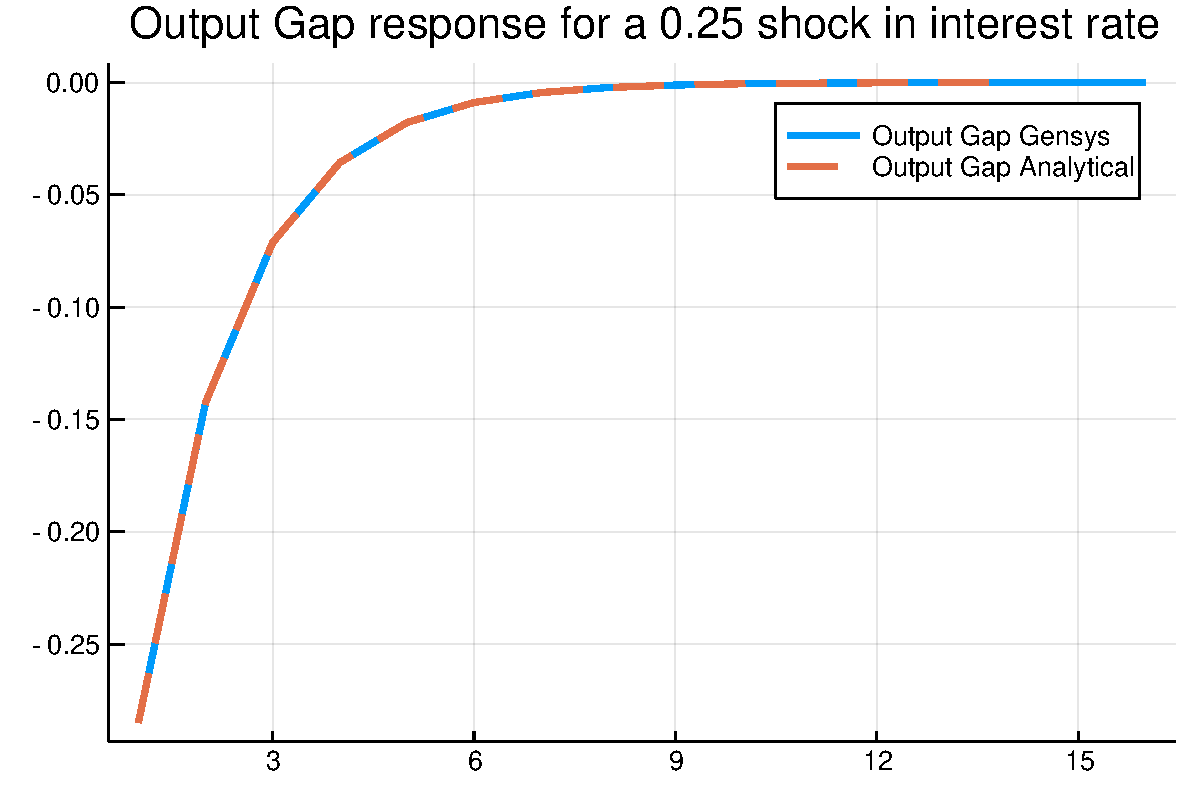
\includegraphics[width=\linewidth]{figures/gensys_12_1.pdf}

\begin{lstlisting}
(*@\HLJLnf{plot}@*)(*@\HLJLp{(}@*)(*@\HLJLni{4}@*)(*@\HLJLoB{*}@*)(*@\HLJLn{irfs}@*)(*@\HLJLp{[}@*)(*@\HLJLoB{:}@*)(*@\HLJLp{,}@*)(*@\HLJLni{3}@*)(*@\HLJLp{],}@*) (*@\HLJLn{label}@*) (*@\HLJLoB{=}@*) (*@\HLJLs{"{}Interest}@*) (*@\HLJLs{Rate}@*) (*@\HLJLs{Gensys"{}}@*)(*@\HLJLp{,}@*) (*@\HLJLn{w}@*) (*@\HLJLoB{=}@*) (*@\HLJLni{3}@*)(*@\HLJLp{)}@*)
(*@\HLJLnf{plot!}@*)(*@\HLJLp{(}@*)(*@\HLJLni{4}@*)(*@\HLJLoB{*}@*)(*@\HLJLn{irfs{\_}true}@*)(*@\HLJLp{[}@*)(*@\HLJLni{2}@*)(*@\HLJLoB{:}@*)(*@\HLJLni{15}@*)(*@\HLJLp{,}@*)(*@\HLJLni{3}@*)(*@\HLJLp{],}@*) (*@\HLJLn{label}@*) (*@\HLJLoB{=}@*) (*@\HLJLs{"{}Interest}@*) (*@\HLJLs{Rate}@*) (*@\HLJLs{Analytical"{}}@*)(*@\HLJLp{,}@*) (*@\HLJLn{line}@*) (*@\HLJLoB{=}@*) (*@\HLJLsc{:dash}@*)(*@\HLJLp{,}@*) (*@\HLJLn{w}@*) (*@\HLJLoB{=}@*) (*@\HLJLni{3}@*)(*@\HLJLp{)}@*)
(*@\HLJLnf{title!}@*)(*@\HLJLp{(}@*)(*@\HLJLs{"{}Nominal}@*) (*@\HLJLs{Interest}@*) (*@\HLJLs{response}@*) (*@\HLJLs{for}@*) (*@\HLJLs{a}@*) (*@\HLJLs{0.25}@*) (*@\HLJLs{shock}@*) (*@\HLJLs{in}@*) (*@\HLJLs{interest}@*) (*@\HLJLs{rate"{}}@*)(*@\HLJLp{)}@*)
\end{lstlisting}

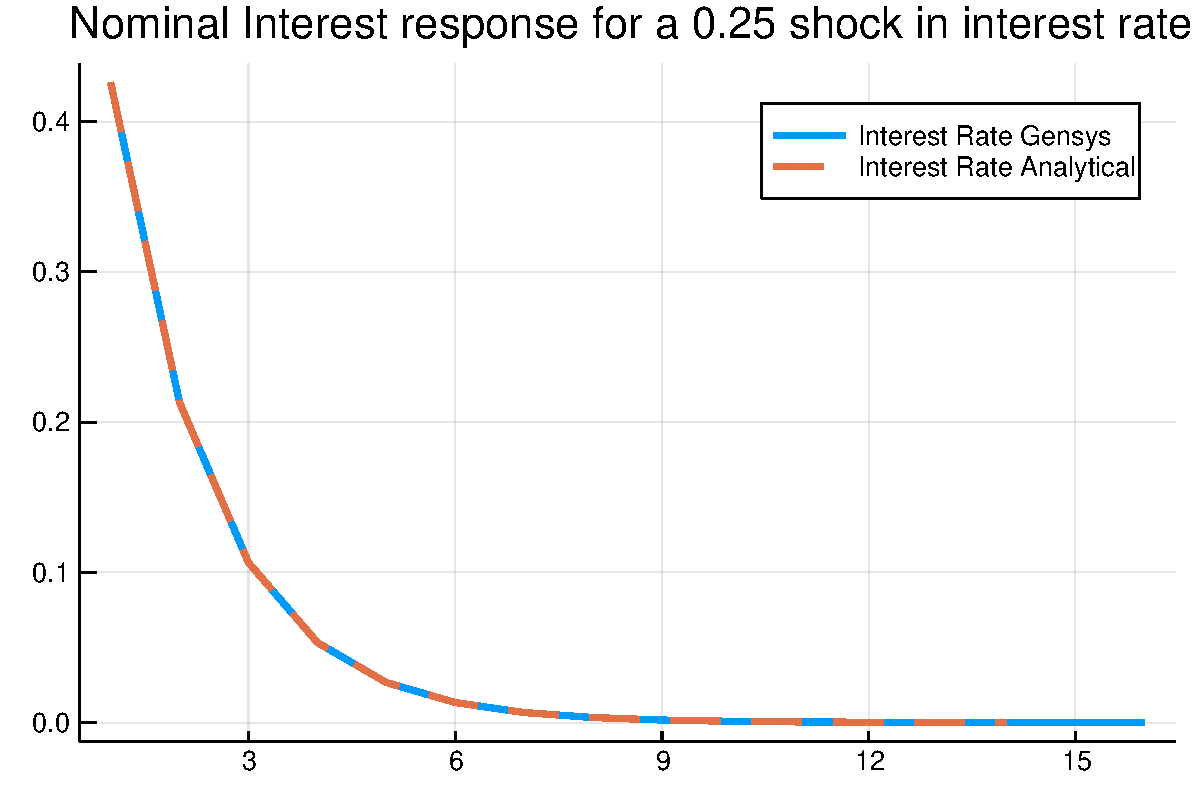
\includegraphics[width=\linewidth]{figures/gensys_13_1.pdf}

\begin{lstlisting}
(*@\HLJLnf{plot}@*)(*@\HLJLp{(}@*)(*@\HLJLn{irfs}@*)(*@\HLJLp{[}@*)(*@\HLJLoB{:}@*)(*@\HLJLp{,}@*)(*@\HLJLni{4}@*)(*@\HLJLp{],}@*) (*@\HLJLn{label}@*) (*@\HLJLoB{=}@*) (*@\HLJLs{"{}v}@*) (*@\HLJLs{Gensys"{}}@*)(*@\HLJLp{,}@*) (*@\HLJLn{w}@*) (*@\HLJLoB{=}@*) (*@\HLJLni{3}@*)(*@\HLJLp{)}@*)
(*@\HLJLnf{plot!}@*)(*@\HLJLp{(}@*)(*@\HLJLn{irfs{\_}true}@*)(*@\HLJLp{[}@*)(*@\HLJLni{2}@*)(*@\HLJLoB{:}@*)(*@\HLJLni{15}@*)(*@\HLJLp{,}@*)(*@\HLJLni{4}@*)(*@\HLJLp{],}@*) (*@\HLJLn{label}@*) (*@\HLJLoB{=}@*) (*@\HLJLs{"{}v}@*) (*@\HLJLs{Analytical"{}}@*)(*@\HLJLp{,}@*) (*@\HLJLn{line}@*) (*@\HLJLoB{=}@*) (*@\HLJLsc{:dash}@*)(*@\HLJLp{,}@*) (*@\HLJLn{w}@*) (*@\HLJLoB{=}@*) (*@\HLJLni{3}@*)(*@\HLJLp{)}@*)
(*@\HLJLnf{title!}@*)(*@\HLJLp{(}@*)(*@\HLJLs{"{}v}@*) (*@\HLJLs{response}@*) (*@\HLJLs{for}@*) (*@\HLJLs{a}@*) (*@\HLJLs{0.25}@*) (*@\HLJLs{shock}@*) (*@\HLJLs{in}@*) (*@\HLJLs{interest}@*) (*@\HLJLs{rate"{}}@*)(*@\HLJLp{)}@*)
\end{lstlisting}

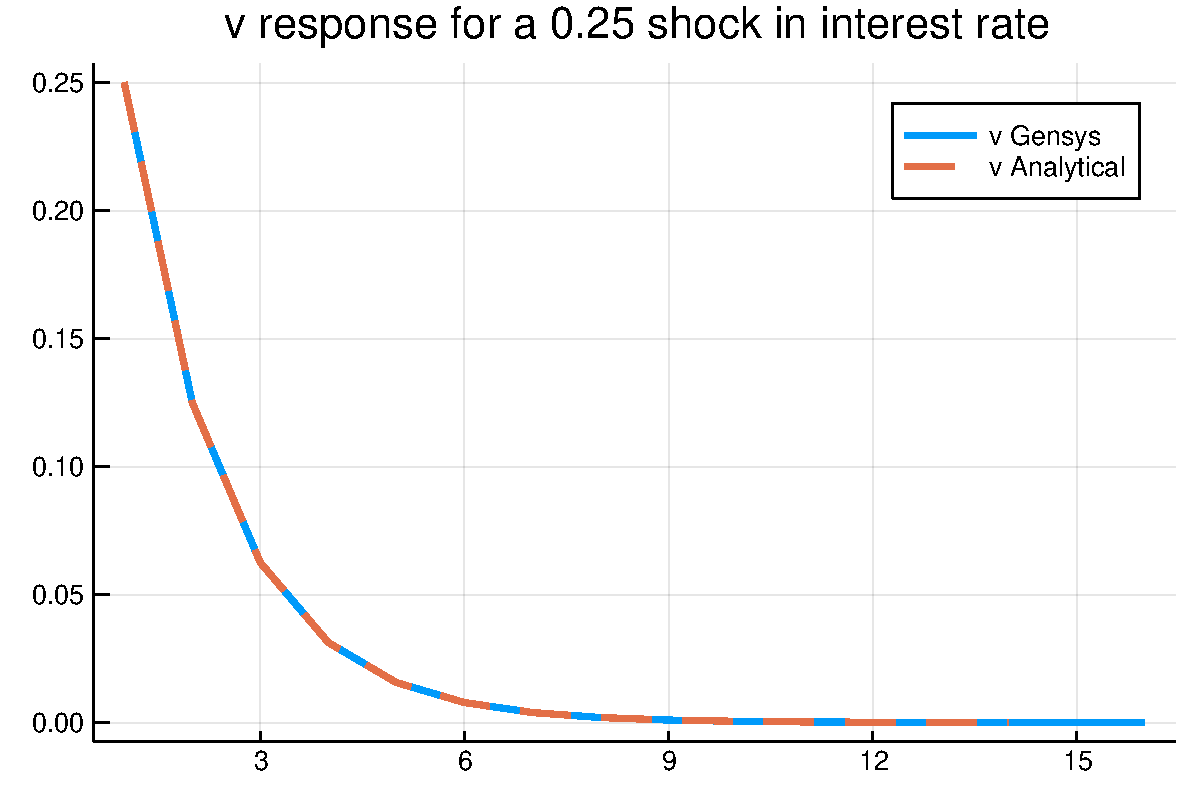
\includegraphics[width=\linewidth]{figures/gensys_14_1.pdf}

The impulse response are identical between the two methods, which is a strong evidence of the reliability and precision of our implementation of Gensys, Gensys itself and Julia capabilities to handle linear algebra routines.



\end{document}
